\documentclass{book}
\usepackage{physics}
\usepackage{graphicx}
\usepackage{caption}
\usepackage{amsmath}
\usepackage[shortlabels]{enumitem}
\usepackage[left=1in,right=1in,top=1in,bottom=1in]{geometry}
\usepackage{bm}
\usepackage{authblk}
\usepackage{empheq}
\usepackage{amsfonts}
\usepackage{esint}
\usepackage[makeroom]{cancel}
\usepackage{dsfont}
\usepackage{framed}
\usepackage{centernot}
\usepackage{mathtools}
\usepackage{bigints}
\usepackage{amsthm}
\theoremstyle{definition}
\newtheorem{defn}{Definition}[section]
\newtheorem{prop}{Proposition}[section]
\newtheorem{rmk}{Remark}[section]
\newtheorem{thm}{Theorem}[section]
\newtheorem{exmp}{Example}[section]
\newtheorem{prob}{Problem}[section]
\newtheorem{sln}{Solution}[section]
\newtheorem*{prob*}{Problem}
\newtheorem{exer}{Exercise}[section]
\newtheorem*{exer*}{Exercise}
\newtheorem*{sln*}{Solution}
\usepackage{empheq}
\usepackage{hyperref}
\usepackage{tensor}
\usepackage{xcolor}
\hypersetup{
	colorlinks,
	linkcolor={black!50!black},
	citecolor={blue!50!black},
	urlcolor={blue!80!black}
}

\newcommand{\diag}{\text{diag}}
\newcommand{\psirot}{\ket{\psi_\text{rot}(t)} }
\newcommand{\RWA}{\ham_\text{rot}^\text{RWA}}


\newcommand{\lambdabar}{{\mkern0.75mu\mathchar '26\mkern -9.75mu\lambda}}



\newcommand*\widefbox[1]{\fbox{\hspace{2em}#1\hspace{2em}}}

\newcommand{\p}{\partial}
\newcommand{\R}{\mathbb{R}}
\newcommand{\C}{\mathbb{C}}
\newcommand{\lag}{\mathcal{L}}
\newcommand{\nn}{\nonumber}
\newcommand{\ham}{\mathcal{H}}
\newcommand{\M}{\mathcal{M}}
\newcommand{\I}{\mathcal{I}}
\newcommand{\K}{\mathcal{K}}
\newcommand{\F}{\mathcal{F}}
\newcommand{\w}{\omega}
\newcommand{\lam}{\lambda}
\newcommand{\al}{\alpha}
\newcommand{\be}{\beta}
\newcommand{\x}{\xi}


\newcommand{\Else}{\text{else}}
\newcommand{\N}{\mathcal{N}}


\newcommand{\sig}{\bm\sigma}
\newcommand{\n}{\mathbf{n}}
\newcommand{\X}{\mathbf{X}}
\newcommand{\s}{\mathbf{S}}

\newcommand{\G}{\mathcal{G}}

\newcommand{\f}[2]{\frac{#1}{#2}}

\newcommand{\ift}{\infty}

\newcommand{\lp}{\left(}
\newcommand{\rp}{\right)}

\newcommand{\lb}{\left[}
\newcommand{\rb}{\right]}

\newcommand{\lc}{\left\{}
\newcommand{\rc}{\right\}}


\newcommand{\V}{\mathbf{V}}
\newcommand{\U}{\mathbf{U}}
\newcommand{\Id}{\mathbb{I}}
\newcommand{\D}{\mathcal{D}}
\newcommand{\Z}{\mathbf{Z}}
\newcommand{\had}{\mathbf{H}}
\newcommand{\Y}{\mathbf{Y}}
%\setcounter{chapter}{-1}


\makeatletter
\renewcommand{\@chapapp}{Chapter}
%\renewcommand\thechapter{$\bf{\ket{\arabic{chapter}}}$}
%\renewcommand\thesection{$\bf{\ket{\arabic{section}}}$}
%\renewcommand\thesubsection{$\bf{\ket{\arabic{subsection}}}$}
%\renewcommand\thesubsubsection{$\bf{\ket{\arabic{subsubsection}}}$}
\makeatother



\usepackage{subfig}
\usepackage{listings}
\captionsetup[lstlisting]{margin=0cm,format=hang,font=small,format=plain,labelfont={bf,up},textfont={it}}
\renewcommand*{\lstlistingname}{Code \textcolor{violet}{\textsl{Mathematica}}}
\definecolor{gris245}{RGB}{245,245,245}
\definecolor{olive}{RGB}{50,140,50}
\definecolor{brun}{RGB}{175,100,80}
\lstset{
	tabsize=4,
	frame=single,
	language=mathematica,
	basicstyle=\scriptsize\ttfamily,
	keywordstyle=\color{black},
	backgroundcolor=\color{gris245},
	commentstyle=\color{gray},
	showstringspaces=false,
	emph={
		r1,
		r2,
		epsilon,epsilon_,
		Newton,Newton_
	},emphstyle={\color{olive}},
	emph={[2]
		L,
		CouleurCourbe,
		PotentielEffectif,
		IdCourbe,
		Courbe
	},emphstyle={[2]\color{blue}},
	emph={[3]r,r_,n,n_},emphstyle={[3]\color{magenta}}
}


\begin{document}
	\begin{titlepage}\centering
		\clearpage
		\title{{\textsc{\textbf{ULTRACOLD FERMI GAS}}}\\ \smallskip - A Quick Guide - \\}
		\author{\bigskip Huan Q. Bui}
		\affil{Massachusetts Institute of Technology}
		\date{\today}
		\maketitle
		\thispagestyle{empty}
	\end{titlepage}




\subsection*{Preface}
\addcontentsline{toc}{subsection}{Preface}

Greetings, \\

This is my personal ``cheatsheet'' for BEC1 experiment with strongly interacting Fermi gas (ironic, I know, but there's a lot of history behind this irony). All information relevant to what I do in the lab plus what I find interesting is accumulated here. \\

\noindent Enjoy!

\newpage
\tableofcontents
\newpage





%%%%%%%%%%%%%%%%%%%%%%%%%%%%%%%%%%%%%%%%%%%%%%
%%%%%%%%%%%%%%%%%%%%%%%%%%%%%%%%%%%%%%%%%%%%%%



\chapter{Ideal Fermi Gas}


\section{Thermodynamics of a non-relativistic gas}

For a non-relativistic gas of particles with spin $s$ in three dimensions with $\mathcal{E}(\vec{k}) = \hbar^2k^2/2m$, we have 
\begin{align*}
	\be P_\eta &= \f{g}{\lambda^3} f^\eta_{5/2}(z) \\
	n_\eta &= \f{g}{\lambda^3} f_{3/2}^\eta(z)\\
	\epsilon_\eta &= \f{3}{2}P_\eta
\end{align*}
with $g = 2s+1$ is the spin degeneracy factor, $z$ is the fugacity parameter $e^{\be \mu}$, and $\eta = -1$ for fermions and $\eta = 1$ for bosons, and 
\begin{align*}
	f_m^\eta(z) = \f{1}{(m-1)!} \int_0^\infty \f{dx\, x^{m-1}}{ z^{-1} e^x - \eta }. 
\end{align*}
The three equations above completely describe the thermodynamics of ideal quantum gases as a function of $z$. To rewrite these equations in terms of the density $n_\eta$, we have to express $f^\eta_m(z)$ in terms of $n_\eta$. To do this, we have to expand $f^\eta_m(z)$ in terms of $z$ in the high temperature limit. The details of this procedure can be found in Chapter 7 of \cite{kardar2007statistical}.  \\

One of the main corollaries of the expansion is that the natural dimensionless expansion parameter 
\begin{align*}
	\f{n_\eta \lambda^3}{g} 
\end{align*}
appears. Here, $\lambda = \sqrt{h^2/2\pi mk_BT}$ is the de Broglie wavelength. For example,
\begin{align*}
	P_\eta = n_\eta k_B T \lb 1 - \f{\eta}{2^{5/2}}\lp \f{n_\eta \lambda^3}{g} \rp + \dots \rb
\end{align*}

We see that quantum mechanical effects become important in the regime where $n_\eta \lambda^3 \geq g \sim 1$. This is called the \textbf{quantum degenerate limit}. Fermi and Boses gases behave very differently in this limit of high density and low temperature. In this document, we will focus mostly on fermions. 


\section{Thermodynamics of an ideal fermi gas}

In the quantum degeneracy limit, fermions obey Fermi-Dirac statistics. The average occupation number as a function of momentum (or energy) is 
\begin{align*}
	\langle n(\vec{k}) \rangle = \f{1}{ e^{(\mathcal{E}(\vec{k}) - \mu)/k_B T} + 1} \xrightarrow{T\to 0} \begin{cases}
		1 \quad \text{ if } \mathcal{E} < \mu\\ 
		0 \quad \text{ if } \mathcal{E} \geq \mu
	\end{cases}
\end{align*}
Here $\mu$ is the chemical potential and $\mathcal{E}(\vec{k})$ is the energy. We see that $\mu$ is a limiting value for $\mathcal{E}(\vec{k})$ (at zero temperature), and call it the \textbf{Fermi energy} $\mathcal{E}_F$. At $T\to 0$, all one-particle states of energy less than $\mathcal{E}_F$ are occupied, forming a \textbf{Fermi sea}. 


\begin{figure}[!htb]
	\centering
	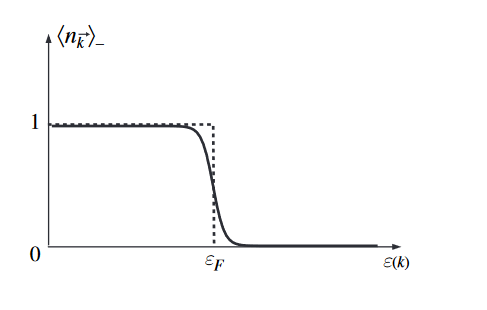
\includegraphics[scale=0.8]{figures/fermi_dist.png}
\end{figure}


\noindent For an ideal Fermi gas, 
\begin{align*}
	\mathcal{E}(\vec{k}) = \f{\hbar^2 k^2}{2m} \implies \mathcal{E}_F \coloneqq \f{\hbar^2 k_F^2}{2m}
\end{align*}
where $k_F$ is the \textbf{Fermi wavenumber}. The Fermi wavenumber $k_F$ can be computed from the number density as:
\begin{align*}
	n = \int_{k < k_F} g \times  \f{d^3 \vec{k}}{(2\pi)^3} =  g\int_{k< k_F} 4\pi k^2 \f{dk}{(2\pi)^3} = \f{g}{6\pi^2}k_F^3.
\end{align*}
So,
\begin{align*}
	\boxed{k_F = \lp \f{6\pi^2 n}{g} \rp^{1/3} \implies \mathcal{E}_F = \f{\hbar^2}{2m} \lp \f{6\pi^2 n}{g} \rp^{2/3}}
\end{align*}

To extract thermodynamics properties of the degenerate Fermi gas in three dimensions (untrapped), we consider the high-$z$ limit of $f_m^-(z)$. Again, Chapter 7 of \cite{kardar2007statistical} shows the details of the various expansions. The result is the \textbf{Sommerfeld expansion}:
\begin{align*}
	\lim_{z\to \infty} f_m^-(z) = \f{(\ln z)^m}{m!} \lb 1 + \f{\pi^2}{6}  \f{m(m-1)}{(\ln z)^2} + \f{7\pi^4}{360} \f{m(m-1)(m-2)(m-3)}{(\ln z)^4} + \dots \rb
\end{align*} 
From the $n_\eta$ equation in the previous section, we find that in the degenerate limit, the density and chemical potential are related by 
\begin{align*}
	\f{n\lambda^3}{g} = f_{3/2}^{-}(z) = \f{(\ln z)^{3/2} }{(3/2)!}\lb 1 + \f{\pi^2}{6}\f{3}{2}\f{1}{2}(\ln z)^{-2}  + \dots \rb \gg 1
\end{align*}

\begin{figure}[!htb]
	\centering
	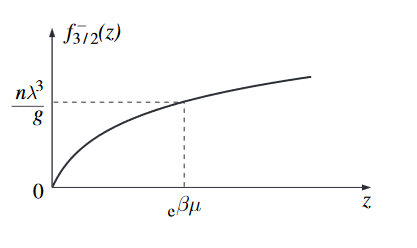
\includegraphics[scale=0.8]{figures/chem_pot.png}
\end{figure}

To lowest order, we have
\begin{align*}
	\lim_{T\to 0} \ln z = \lp \f{3}{4\sqrt{\pi}} \f{n\lambda^3}{g} \rp^{2/3} = \f{\be \hbar^2}{2m} \lp \f{6\pi^2 n}{g} \rp^{2/3} = \be \mathcal{E}_F \implies \lim_{T\to 0} \mu = \mathcal{E}_F
\end{align*}
which is what we found earlier by looking at the mean occupation number for fermions. \\



At finite but small temperatures, we have corrections:
\begin{align*}
	\ln z \approx \be \mathcal{E}_F \lb 1 - \f{\pi^2}{12} \lp \f{k_B T}{\mathcal{E}_F} \rp^2 + \dots \rb
\end{align*}

\begin{figure}[!htb]
	\centering
	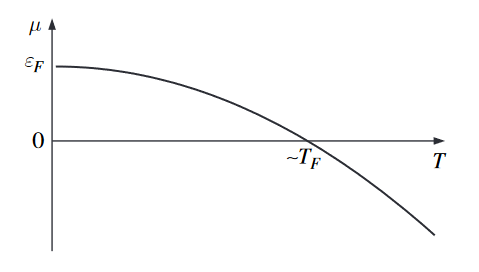
\includegraphics[scale=0.8]{figures/chem_pot_v_T.png}
\end{figure}

We see that the chemical potential $\mu = k_B T \ln z$ is positive at low temperature and negative at high temperature. It changes sign at $T \sim T_F = \mathcal{E}_F/k_B$. \\


Using a similar approach, one finds the low-temperature expansion for pressure:
\begin{align*}
	\be P = \be P_F\lb 1 + \f{5}{12}\pi^2 \lp \f{k_B T}{\mathcal{E}_F} \rp^2 + \dots \rb, \quad\quad \boxed{P_F = \f{2}{5}n \mathcal{E}_F}
\end{align*}
Here $P_F$ is the \textbf{fermi pressure}. Note that the fermi gas at zero temperature has nonzero pressure and internal energy, unlike its classical counterpart. 

\begin{figure}[!htb]
	\centering
	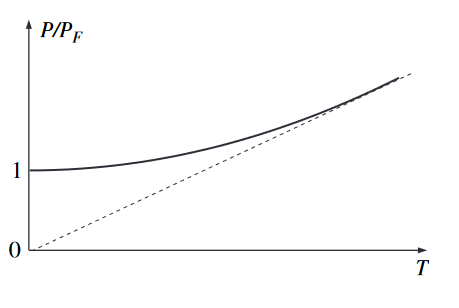
\includegraphics[scale=0.8]{figures/fermi_pressure.png}
\end{figure}

The internal energy (density) is obtained from the third equation in the previous section: 
\begin{align*}
	\boxed{\epsilon = \f{E}{V} = \f{3}{2}P = \f{3}{5}nk_B T_F \lb 1 + \f{5}{12}\pi^2 \lp \f{k_B T}{\mathcal{E}_F} \rp^2 + \dots \rb}
\end{align*}

From here, one finds the low-temperature heat capacity:
\begin{align*}
	C_V = \f{dE}{dT} = \f{\pi^2}{2}Nk_B \lp \f{T}{T_F} \rp + \mathcal{O}\lp \f{T}{T_F}  \rp^3
\end{align*}

\begin{figure}[!htb]
	\centering
	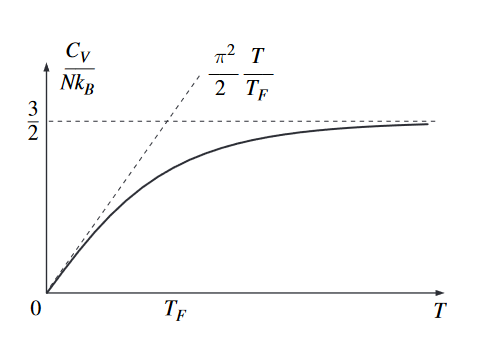
\includegraphics[scale=0.8]{figures/heat_cap.png}
\end{figure}


Note: the linear scaling of $C_V$ as $T\to 0$ is a general feature of a fermi gas and is valid in all dimensions. The physical interpretation is as follows: At small temperatures, all single-particle states are occupied. As a result, only particles within a distance of about $k_B T$ of the fermi energy can be thermally excited. This represents only a small fraction $(T/T_F)$ of the fermions. Each excited particle gains $k_B T$, leading to a change in $E$ of $k_B T N (T/T_F)$. So $C_V \propto dE/dT \sim N k_BT/T_F$ which is linear in $T$. This conclusion is also \textbf{valid for interacting fermi gases}. 



\section{Ideal Fermi gas in a harmonic trap}

See next chapter. This section is more naturally treated in conjunction with a number of related topics.


\chapter{Interacting Fermi Gas}


\section{Hyperfine Structure}

\section{Collisional Properties}


\section{Cooling and Trapping techniques}


\section{RF Spectroscopy}


\section{Feshbach resonance}

This section is adapted from \cite{campbellfeshbach} and \cite{ketterle2008making}.


\subsection{Scattering theory}




It is necessary to have some basic understanding of scattering theory before having an intuitive picture of Feshbach resonance. Our main focus here is \textbf{low-energy scattering}, so we will not discuss Born perturbative series expansion method for high-energy scattering and instead look at method of partial waves.\\

Let's begin. There are three types of scattering processes: elastic, inelastic, and absorption. We will be focusing on \textbf{elastic scattering} where both the energy and particle number are conserved.  \\


\subsubsection{Scattering cross section}


The main concept in scattering theory is the \textbf{differential cross section}, $d\sigma$, which characterizes scattering processes. $d\sigma$ has units of area. Consider a stream of particles with flux $j$ (in units of particles per unit time per unit area) hitting some detector which measures the number of particles $N\,d\Omega$ per unit time scattered into an element of solid angle $d\Omega$. We must then have
\begin{align*}
	j\,d\sigma = N\, d\Omega.
\end{align*}
Rearranging gives
\begin{align*}
	d\sigma = \f{N}{j}\, d\Omega
\end{align*}
From here we can integrate to find the \textbf{total differential cross section}:
\begin{align*}
	\sigma = \int \f{d\sigma}{d\Omega} \,d\Omega = \int_0^{2\pi}d\phi\, \int_0^\pi d\theta \sin\theta \f{d\sigma}{d\Omega}.
\end{align*}
As we will see, this quantity depends on the energy of incoming particles. The cross section is an effective area for collision.

\subsubsection{Classical scattering}

In most cases, we have concerned with scattering against a \textbf{central potential} $V(r)$. Consider the quantity $N\,d\Omega$ again. This quantity is the number of particles per unit time scattered between $\theta$ and $\theta+d\theta$ (large grey area). By conservation of particle number, it must be equal to the flux $j$ multiplied by the area of the small grey area given by $2\pi b \,db$:
\begin{align*}
	N\,d\Omega = 2\pi \sin\theta\,d\theta N = 2\pi b\,db \,j
\end{align*}  

\begin{figure}[!htb]
	\centering
	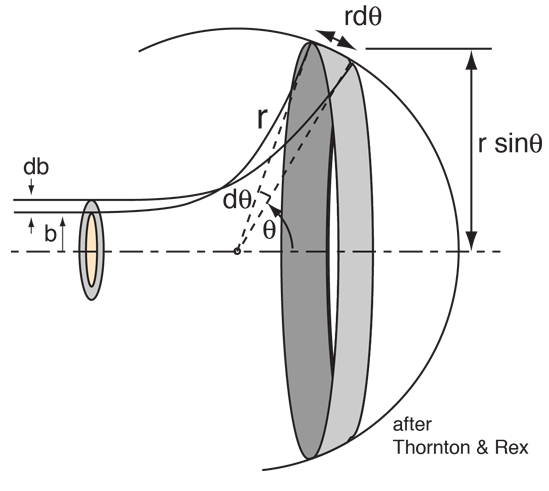
\includegraphics[scale=1.5]{figures/Ruthcross.png}
\end{figure}

By azimuthal symmetry, we see that $b = b(\theta)$. This quantity is called the \textbf{impact parameter}. It is the perpendicular distance to the closest approach if the projectile were undeflected. For every deflection angle $\theta$, there is an associated impact parameter. Hence $b = b(\theta)$. \\


From the equation above, we obtain
\begin{align*}
	\f{d\sigma(\theta)}{d\Omega} = \f{b}{\sin\theta} \abs{\f{db}{d\theta}}
\end{align*}

\noindent \underline{Example}: For hard sphere scattering, the impact parameter is 
\begin{align*}
	b(\theta) = R\sin\al = R\sin \lp \f{\pi - \theta}{2} \rp = -R\cos(\theta/2).
\end{align*}
This gives
\begin{align*}
	\f{d\sigma(\theta)}{d\Omega} = \f{R^2}{4} \implies \sigma = \pi R^2,
\end{align*}
as expected. The cross section for hard sphere scattering is simply the cross sectional area of the sphere. \qed\\

\begin{figure}[!htb]
	\centering
	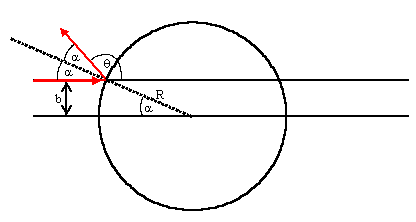
\includegraphics[scale=0.5]{figures/hard_sphere.png}
\end{figure}



\noindent \underline{Example}: Here we look at classical Coulomb scattering with the central potential:
\begin{align*}
	V(r) = \f{\kappa}{r}.
\end{align*}
In this case, 
\begin{align*}
	\f{d\sigma}{d\Omega} = \f{b}{\sin\theta} \abs{\f{db}{d\theta}} = \f{\kappa^2}{16 E^2} \f{1}{\sin^4 \theta/2}.
\end{align*}
This is the famous \textbf{Rutherford formula}. \qed



\subsubsection{Quantum scattering}

The setup here is same as before. We are interested in the steady state of the scattering problem (think of this as having a constant stream of incoming particles/waves and ignore the "encounter period").
\begin{figure}[!htb]
	\centering
	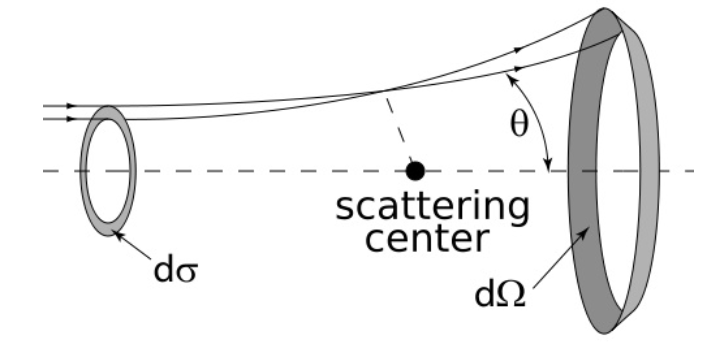
\includegraphics[scale=0.4]{figures/scat_center.png}
\end{figure}
The total wavefunction of incoming and scattered particles must solve the Schr\"{o}dinger equation:
\begin{align*}
	E\psi(\vec{r}) = -\lb \f{\hbar^2}{2m}\nabla^2 + V(r)\rb \psi(\vec{r}). 
\end{align*}
Let the incoming wave be a plane wave 
\begin{align*}
	\psi_\text{inc} = e^{i\vec{k}\dot \vec{r}}
\end{align*}
Then the outgoing wave at large $r$ may be written as 
\begin{align*}
	\psi_\text{out} = f(\theta) \f{e^{ikr}}{r}.
\end{align*}
And so the total wavefunction may be written as
\begin{align*}
	\boxed{\psi(\vec{r}) = e^{i\vec{k}\cdot \vec{r}} + f(\theta) \f{e^{ikr}}{r}, \quad\quad r \gg L} 
\end{align*}
where $L$ is some effective range of the potential. By writing down the full wavefunction in the partial wave expansion, one may find that
\begin{align*}
	f(\theta) = \sum_{l=0}^\infty (2l+1) f_l(k) P_l(\cos\theta)
\end{align*}
where
\begin{align*}
	f_l(k) = \f{e^{2i\delta_l(k)} - 1}{2ik} = \f{e^{i\delta_l(k)}}{k} \sin\delta_l
\end{align*}
are the \textbf{partial wave scattering amplitudes}, which are defined by the \textbf{phase shifts} $\delta_l(k)$. \\

Now we want to relate the scattering amplitude to cross section. To do this, we have to find the particle flux. By definition:
\begin{align*}
	\vec{j} = -i \f{\hbar}{m}\Re\lb \psi^* \nabla \psi \rb \approx \f{\hbar \vec{k}}{m} + \f{\hbar k}{m}\hat{e}_r \f{|f(\theta)|^2}{r^2} + \dots
\end{align*}
after neglecting rapidly fluctuation contributions. With this, we can compute:
\begin{align*}
	N\,d\Omega = (\vec{j}\cdot \hat{e}_r) r^2\,d\Omega = \f{\hbar k}{m} |f(\theta)|^2\,d\Omega + \dots 
\end{align*}
But we also know that this flux $N\,d\Omega$ must be equal to the incoming flux $j_I \,d\sigma = (\hbar k/m)\,d\sigma$ (plane wave incoming flux). So,
\begin{align*}
	N\,d\Omega = j_I \,d\sigma \implies d\sigma = |f(\theta)|^2\,d\Omega \implies \boxed{ {\f{d\sigma}{d\Omega} = |f(\theta)|^2}}
\end{align*}
From here and the definition for $f(\theta)$, we can calculate the total cross section:
\begin{align*}
	\sigma_\text{tot} = \int d\sigma = \int |f(\theta)|^2\, d\Omega = \dots = 4\pi \sum_{l}(2l+1) |f_l(k)|^2 = \f{4\pi}{k^2}\sum_{l=0}^\infty (2l+1)\sin^2\delta_l(k),
\end{align*}
where we have used the definition of $f_l(k)$ in the last equality. A consequence of this is that
\begin{align*}
	\Im f(0) = \f{k}{4\pi} \sigma_\text{tot}.
\end{align*}
This is the \textbf{optical theorem}, which encapsulate particle conservation.

\begin{framed}
	In summary, the quantum scattering cross section is fully characterized by the scattering amplitude $f(\theta)$, which implicitly depends on the energy $E=E(k)$ in its partial wave expansion. The partial wave amplitudes $f_l(k)$ in these expansions are ultimately defined by the phase shifts $\delta_l(k)$.
\end{framed}


The next step is therefore to find the phase shifts.  To do this we need the \textbf{method of partial waves}, where we start by decomposing the full wavefunction into, well, partial waves:
\begin{align*}
	\psi(\vec{r}) = \sum_{l=0}^\infty R_l(r) P_l(\cos\theta). 
\end{align*}
From the Schr\"{o}dinger equation for the scattering wavefunction with $E = \hbar^2 k^2 / 2m$ (energy of the incoming wave), we find the radial equation
\begin{align*}
	\lb -\f{\hbar^2}{2m}\lp \p_r^2 + \f{2}{r}\p_r - \f{l(l+1)}{r^2} \rp + V(r) \rb R_l(r) = \f{\hbar^2 k^2}{2m} R_l(r).
\end{align*}
Rearranging this gives
\begin{align*}
	\lb \p_r^2 + \f{2}{r}\p_r - \f{l(l+1)}{r^2} - U(r) + k^2 \rb R_l(r) = 0
\end{align*}
with $U(r) = 2mV(r)/\hbar^2$.\\

Provided that the potential is sufficiently short-ranged, the scattering wavefunction is a superposition of incoming and outgoing spherical waves:
\begin{align*}
	R_l(r) \approx \f{i}{2k} \sum_{l=0}^\infty i^l (2l+1) \lp \f{e^{-i(kr - l\pi/2)}}{r} - e^{2i\delta_l(k)} \f{e^{i(kr - l\pi/2)}}{r} \rp.
\end{align*}
In particular, for $l=0$ ($s$-wave channel):
\begin{align*}
	\boxed{R_0(r) \approx \f{1}{kr} e^{i\delta_0 (k)} \sin(kr + \delta_0(k))}
\end{align*}
At low energy ($kL \ll 1$), the $s$-wave channel dominate. \\

Introducing the \textbf{reduced radial wavefunction} 
\begin{align*}
	u(r) = rR_0(r), \quad u(0) = 0
\end{align*}
we get a simplified radial equation:
\begin{align*}
	\lb \p_r^2 - U(r) + k^2 \rb u(r) = 0.
\end{align*}
We now introduce the \textbf{scattering length} $a_0$, defined by the condition:
\begin{align*}
	u(a_0) = 0, \quad kL\ll 1
\end{align*}
What, then, is $a_0$ in terms of the incoming wave momentum?
\begin{align*}
	0 &= u(a_0)\\
	 &= \sin(ka_0 + \delta_0(k))\\
	 &= \sin(ka_0)\cos(\delta_0(k)) + \cos(ka_0)\sin(\delta_0(k)) \\
	 &= \sin\delta_0(k) \lb \cot \delta_0(k) \sin(ka_0) + \cos(ka_0) \rb\\
	 &\approx \sin \delta_0(k) \lb ka_0 \cot \delta_0(k) + 1 \rb
\end{align*}
Solving this gives
\begin{align*}
	\boxed{a_0 = -\lim_{k\to 0} \f{1}{k}\tan \delta_0(k)}
\end{align*}
To see why $a_0$ is called the scattering length, we can compute the scattering cross section at low energy:
\begin{align*}
	\sigma_\text{tot} =  \f{4\pi}{k^2}\sin^2 \delta_0(k) \xrightarrow{k\to 0} \f{4\pi}{k^2} \f{(ka_0^2)}{1+(ka_0)^2} \approx 4\pi a_0^2.
\end{align*}
We see that $a_0$ \textbf{characterizes the effective size of the target}, and so its nomenclature is justified.\\



\noindent \underline{Example}: \textbf{Quantum hard-sphere scattering.}\\

Consider the hard-sphere potential,
\begin{align*}
	U(r) = \begin{cases}
		\infty \quad r < R \\
		0 \quad r > R
	\end{cases}
\end{align*}
The boundary condition is $u(R) = 0$ (the sphere is impenetrable). From here, the low-energy scattering reduced radial wavefunction is 
\begin{align*}
	u(r) = A\sin(kr + \delta_0), \quad \delta_0 = -kR.
\end{align*}
The scattering length is therefore 
\begin{align*}
	a_0 = -\lim_{k\to 0} \f{1}{k}\tan (-kR) \approx R.
\end{align*}
Since the phase shift is known, we can calculate the scattering amplitude:
\begin{align*}
	f_0(k) = \f{e^{ikR}}{k}\sin(kR).
\end{align*}
The total scattering cross section is therefore
\begin{align*}
	\sigma_\text{tot} \approx 4\pi \f{\sin^2 kR}{k^2} \approx 4\pi R^2
\end{align*}
Notice that the answer is $4\pi R^2$ as opposed to $\pi R^2$ like in the classical case. The factor of 4 enhancement is due to diffraction processes at the sharp potential. \qed\\



\noindent \underline{Example}: \textbf{Scattering by attractive square well.}\\

Here we consider a potential of the form
\begin{align*}
	U(r) = -U_0 \theta(R-r), \quad U_0 > 0
\end{align*}
where $\theta(\dot)$ is the Heavyside step function. We solve the SE in two regions and get 
\begin{align*}
	u(r) = \begin{cases}
		C\sin(Kr) \quad r < R \\
		sin(kr + \delta_0) \quad r > R
	\end{cases}
\end{align*}
where $K^2 = k^2 + U_0 > k^2$ and $\delta_0$ is the scattering phase shift. By matching the solutions and their derivatives at $R$ gives
\begin{align*}
	Csin(KR) = \sin(kR + \delta_0) \quad\quad CK\cos(KR) = k\cos(kR + \delta_0) \implies K\cot(KR) = k\cot(kR+ \delta_0)
\end{align*}
From this, we get
\begin{align*}
	\tan \delta_0 (k)= \f{k\tan(KR) - K\tan(kR)}{K + k\tan(kR)\tan(KR)}, \quad K^2 = k^2 + U_0.
\end{align*}
When $kR \ll 1$ (low energy), $K \approx \sqrt{U_0}$, we find that the scattering length is 
\begin{align*}
	a_0 = -\lim_{k\to 0} \f{1}{k}\tan \delta_0(k) \approx -R \lp \f{\tan(KR)}{KR} - 1 \rp.
\end{align*}
Notice that for $KR < \pi/2$, the scattering length is negative. \textbf{What does the sign of the scattering length represent?} $a_0 > 0$ means the potential is repulsive, while $a_0 < 0$ means the potential is attractive. In this problem, the attractive square potential leads to the $l=0$ phase shift
\begin{align*}
	\delta_0 \approx -ka_0 \approx kR \lp \f{\tan KR}{KR} - 1 \rp
\end{align*}
and total cross section
\begin{align*}
	\sigma_\text{tot} = \f{4\pi}{k^2}\sin^2 \delta_0(k) \approx 4\pi R^2 \lp \f{\tan KR}{KR} - 1 \rp^2, \quad \quad K \approx \sqrt{U_0}
\end{align*}

Let $k$ be fixed and let $U_0$ be tunable. 
\begin{itemize}
	\item If $KR \ll 1$, then $a_0 < 0$, the potential is attractive.
	
	\item If $KR \to \pi/2$, both scattering length and cross section diverge. The influence of the target becomes effectively infinite in range. In this case, the square well just meets the criterion to host a single $s$-wave bound state. 
	
	\item As $KR$ is increased, $a_0$ turns positive, and the potential becomes repulsive until $KR = \pi$ for which $\sigma_\text{tot} = 0$, and the process repeats. 
	
	\item When $KR = n\pi$, the scattering cross section vanishes identically and the target becomes invisible. This is the \textbf{Ramsauer-Townsend effect}.
\end{itemize}


\begin{figure}[!htb]
	\centering
	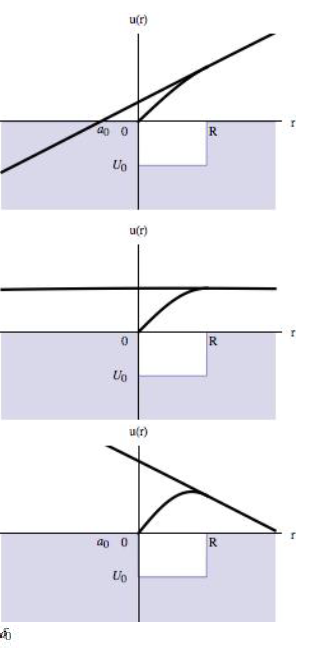
\includegraphics[scale=0.7]{figures/a0.png}
	\caption{Attractive potential, infinite range potential, repulsive potential.}
\end{figure}



We are sensing that at $KR = n\pi/2$ where $n$ is odd, there is a \textbf{resonance} phenomenon. And we would be right. In general, the $l$-th partial cross section is given by 
\begin{align*}
	\sigma_l = \f{4\pi}{k^2}(2l+1) \f{1}{1+ \cot^2\delta_l(k)}, \quad \sigma_\text{tot} = \sum_l \sigma_l.
\end{align*}
The functional form tells us that $\sigma_l$ is peaked whenever $\cot\sigma_l$ vanishes. In fact, as $\sigma_l(k)$ is swept across odd multiples of  $\pi/2$, the cross section exhibits a narrow peak as a function of energy. This is indeed a \textbf{resonance phenomenon}. 





In practice, the metastable bound state form by the particle in the potential has a lifetime defined by $\Gamma(E) = \hbar /\tau$, where $\Gamma(E)$ is the width of the resonance. Near the resonance, the phase shift is related to this width as 
\begin{align*}
	\cot \delta_l(k) = \f{E_R - E}{\Gamma(E)/2}
\end{align*}
where $E_R$ is the resonance energy. It turns that if $\Gamma(E)$ varies slowly in energy, then the partial cross section near resonance is given by the \textbf{Breit-Wigner formula}
\begin{align*}
	\sigma_l(E) = \f{4\pi}{k^2}(2l+1) \f{\Gamma^2(E_R)/4}{(E-E_R)^2 + \Gamma^2(E_R)/4}
\end{align*}
which is a typical resonance profile.

\begin{figure}[!htb]
	\centering
	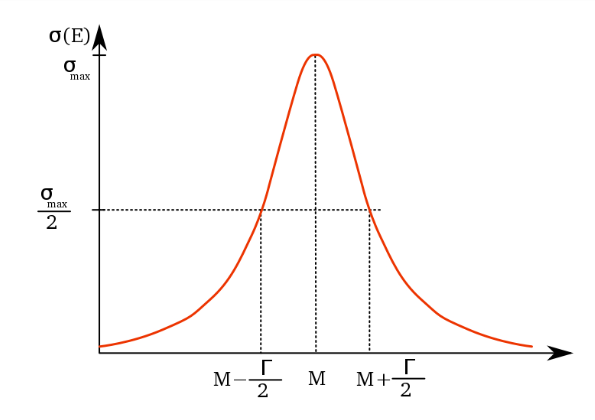
\includegraphics[scale=0.5]{figures/resonance.png}
\end{figure}

\begin{framed}
	Physically, at resonance, the amplitude of the wavefunction within the potential region is high and the probability of finding the scattered particle inside the well is correspondingly high.
\end{framed}


\subsection{Feshbach resonance}

Ultracold atoms interact through the short-ranged van der Walls interaction, whose effetive range can be tuned by allowing particles to form virtual bound state -- a resonance. By adjusting the separation between entrance channel states and bound state through an external magnetic field, the system can be tuned through resonance. This allows the effective interaction to be tuned from repulsive to attractive simply by changing an external field. \\


Consider two fermionic atoms. 


\subsection{FB resonance: Spherical Well Model}

\subsection{FB resonance: Coupled Square Well Model}

\subsection{An intuitive picture}




\section{Analysis of density distributions}













\chapter{Strongly Interacting Fermi Gas}


\bibliographystyle{abbrv} 
\bibliography{BUI_Fermi_refs}% Produces the bibliography via BibTeX.




	
	
\end{document}